\documentclass{article}
\usepackage{graphicx}% Required for inserting images
\usepackage{lindrew}
\usepackage[shortlabels]{enumitem}
\usepackage{pdfpages}
\usepackage{enumerate}
\usepackage{algorithm}
\usepackage{algpseudocode}
\usepackage{matlab-prettifier}
\usepackage{pythonhighlight}

\title{CS 156a Problem Set 7}
\author{Amitesh Pandey}
\date{November 2024}

\begin{document}
\maketitle
\section*{Validation}
The code for all 5 of the following problems is appended at the end. 
\subsection*{Problem 1}
We get 0.0 as the smallest validationt error, obtained with $k =6$ thus $\textbf{[d]}$. 
\subsection*{Problem 2}
We get 0.1 as the smallest out error, obtained with $k = 7$, thus $\textbf{[e]}$.
\subsection*{Problem 3}
We get 0.08 as the smallest validation, obtained with $k = 6$, thus $\textbf{[d]}$.
\subsection*{Problem 4}
We get 0.19 as the smallest out error, obtained with $k = 6$, thus $\textbf{[d]}$.
\subsection*{Problem 5}
Our errors with chosen $k = 6$ for out error are $(0.08, 0.19) \approx (0.1, 0.2)$, closest to $\textbf{[b]}$. 
\section*{Validation Bias}
\subsection*{Problem 6}
For $e_1$ and $e_2$, by definition of uniformly distributed, we have 0.5, 0.5 as the expected values. Now for $e$, we have $\mathbb{P}[e > z] = \mathbb{P}[e_1, e_2 > z]$, since $e_1$ and $e_2$ are independent and uniform, we have $\mathbb{P}[e > z] = (1-z)^{2}$, so the CDF of $e$ is $F_z = 1 - (1-z)^{2}$. Then the PDF is simply $P_z = \frac{\text{d}}{\text{d}z} (F_z) = \frac{\text{d}}{\text{d}z}(1 - (1-z)^{2}) = 2(1-z)$. For the expected value, we know $\mathbb{E}[e] = \int_{0}^{1} zP_z\text{d}z$, which gets us $\mathbb{E}[e] = 2\int_{0}^{1}z(1-z)\text{d}z = 1/3$, our solution is $(0.5, 0.5, 0.33)$ closest to $\textbf{[d]}$. 
\newpage
\section*{Cross Validation}
\subsection*{Problem 7}
We coded up a constant and linear model for all given values of $\rho$ and came to the conclusion that up to 2 decimal places, it is option $\textbf{[c]}$, that results in equal error for both models. 
\section*{PLA vs SVM}
The code for all 3 of the following problems is appended at the end
\subsection*{Problem 8}
We get that 54.6\% of the times, SVM is better than PLA, closest to 60\%, option \textbf{[c]}. 
\subsection*{Problem 9}
We get that 74.1\% of the times, SVM is better than PLA, closest to 65\%, option $\textbf{[d]}$, but barely.
\subsection*{Problem 10}
We get that 2.998 is the average vector length over 1000 experiments, closest to 3, so option $\textbf{[b]}$.

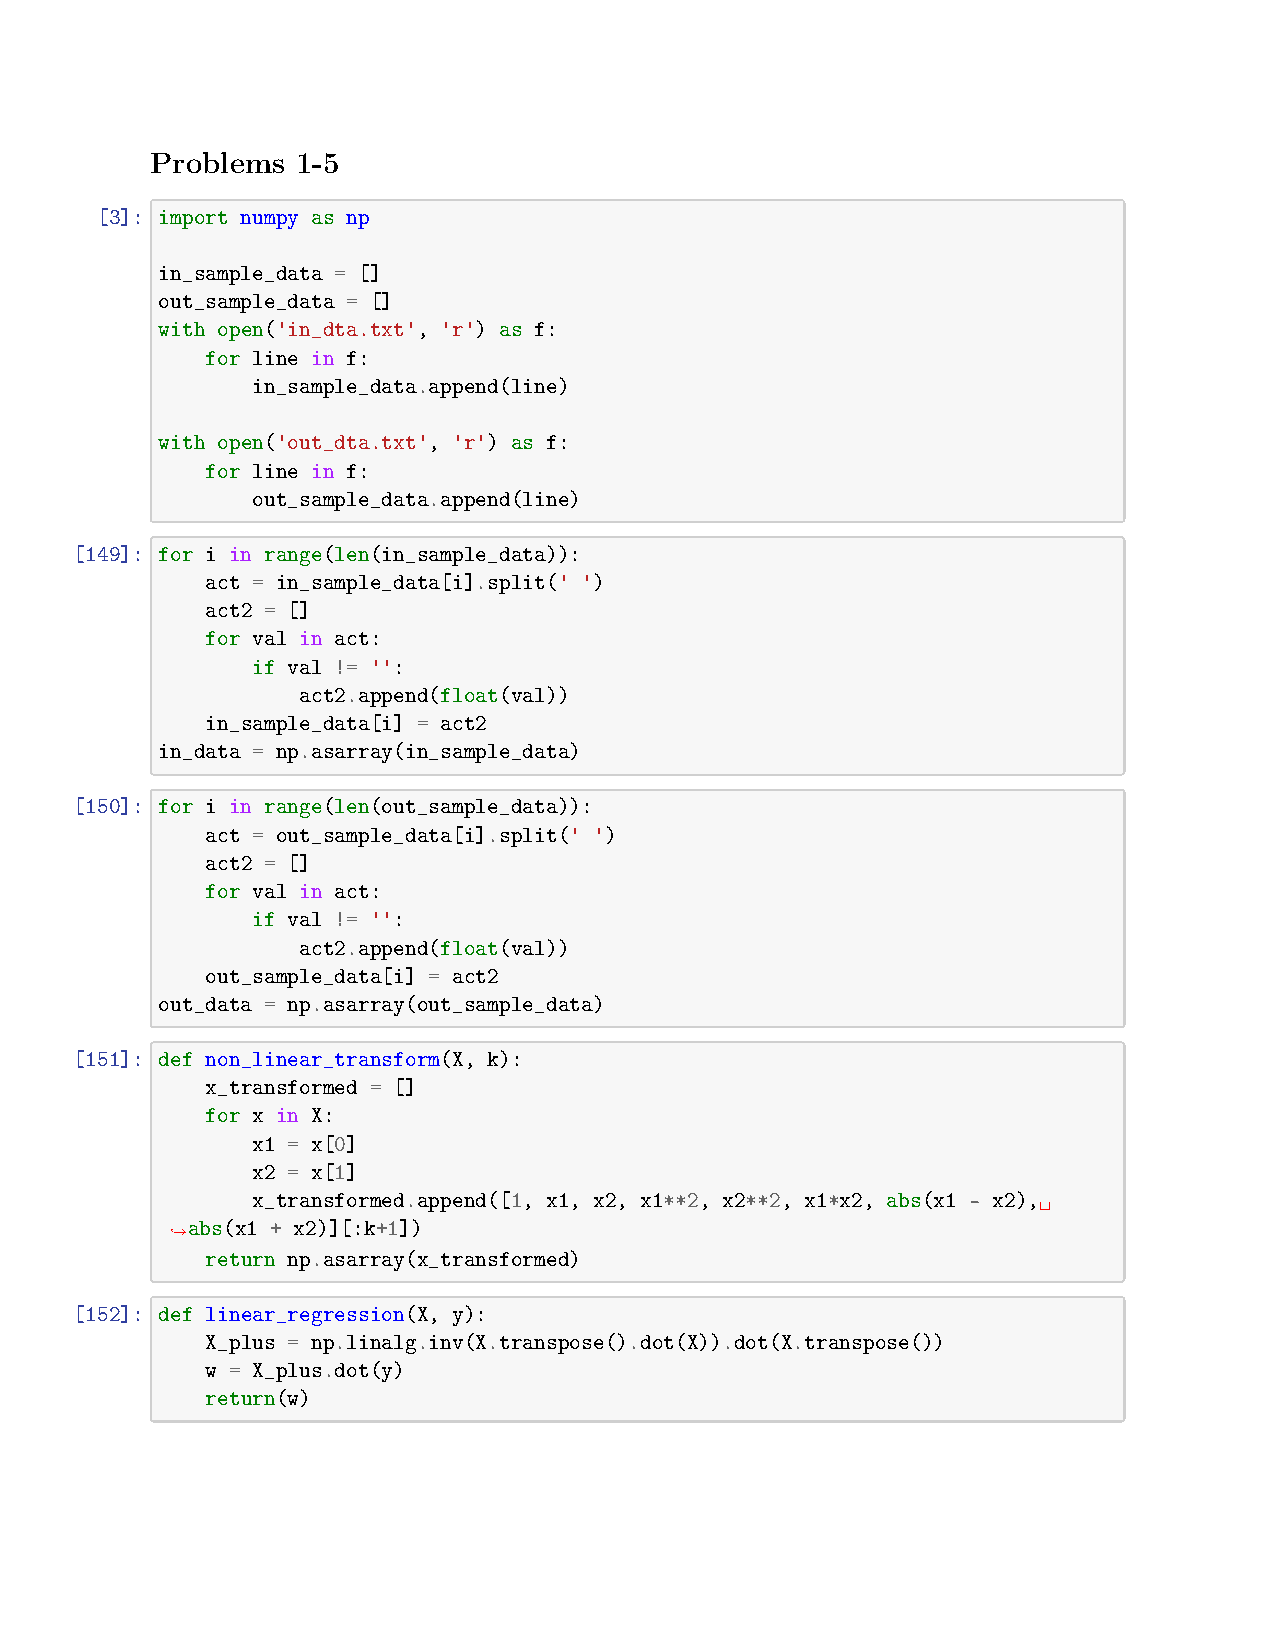
\includepdf[pages=-]{Code_for_HW7.pdf}
\end{document}
